\hypertarget{rcuflashprog_8c}{
\section{rcuflashprog.c File Reference}
\label{rcuflashprog_8c}\index{rcuflashprog.c@{rcuflashprog.c}}
}
Programming tool for the RCU flash memory. 

{\tt \#include $<$stdlib.h$>$}\par
{\tt \#include $<$stdio.h$>$}\par
{\tt \#include $<$string.h$>$}\par
{\tt \#include $<$unistd.h$>$}\par
{\tt \#include \char`\"{}dcsc\-Msg\-Buffer\-Interface.h\char`\"{}}\par
{\tt \#include \char`\"{}framever.h\char`\"{}}\par
{\tt \#include $<$sys/stat.h$>$}\par
{\tt \#include $<$sys/time.h$>$}\par
{\tt \#include $<$rcuflashprog.h$>$}\par


Include dependency graph for rcuflashprog.c:\begin{figure}[H]
\begin{center}
\leavevmode
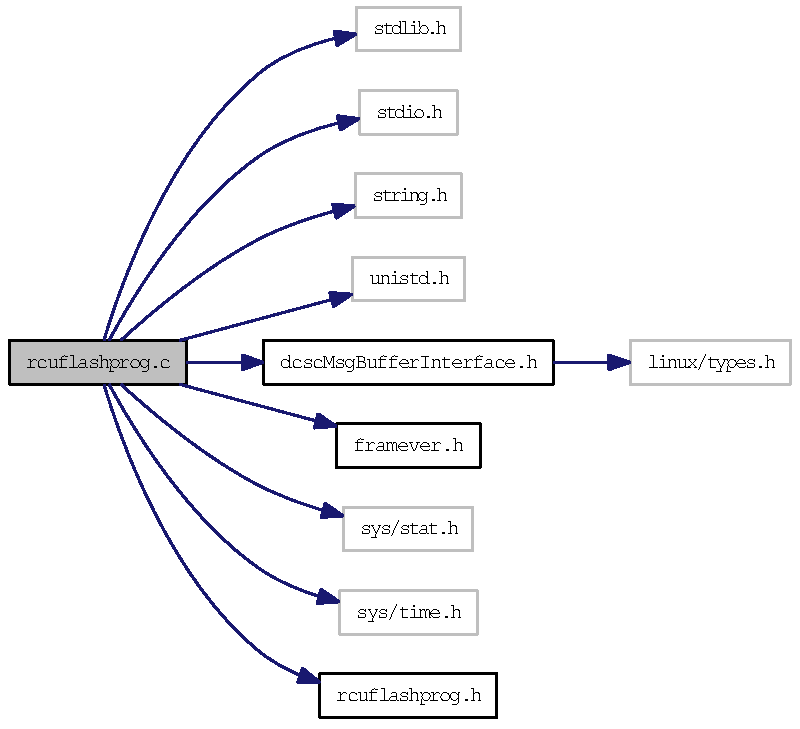
\includegraphics[width=210pt]{rcuflashprog_8c__incl}
\end{center}
\end{figure}
\subsection*{Defines}
\begin{CompactItemize}
\item 
\#define \hyperlink{rcuflashprog_8c_a93f0eb578d23995850d61f7d61c55c1}{FALSE}~0
\item 
\#define \hyperlink{rcuflashprog_8c_a8cecfc5c5c054d2875c03e77b7be15d}{TRUE}~1
\end{CompactItemize}
\subsection*{Functions}
\begin{CompactItemize}
\item 
int \hyperlink{rcuflashprog_8c_3c04138a5bfe5d72780bb7e82a18e627}{main} (int argc, char $\ast$$\ast$argv)
\item 
int \hyperlink{rcuflashprog_8c_237fcbe3877916a856ff7acf973ee2ba}{do\-Flash\-Frame} (char $\ast$conffilename, int \hyperlink{rcuflashprog_8c_a1aabbeb0deebd40a25e329692500bbe}{BB\_\-FLASH})
\begin{CompactList}\small\item\em The programming of the readframes and writeframes is done here. \item\end{CompactList}\item 
void \hyperlink{rcuflashprog_8c_050a67a2d2eae27eb446eafe228a4f3e}{build\-Frame\-Filename} (int $\ast$p\-Frameaddr, char $\ast$pfilename)
\begin{CompactList}\small\item\em The frameaddress is given with the block, major and minor in an int array as the first parameter. \item\end{CompactList}\item 
int \hyperlink{rcuflashprog_8c_cd9a55766b840c98d87b0ce1a76af867}{do\-Scrubbing} (char $\ast$conffilename, int \hyperlink{rcuflashprog_8c_a1aabbeb0deebd40a25e329692500bbe}{BB\_\-FLASH})
\begin{CompactList}\small\item\em Everything needed for a complete scrubbing is done here. \item\end{CompactList}\item 
int \hyperlink{rcuflashprog_8c_017730762068a4d5359376e97dac8257}{do\-Init} (char $\ast$conffilename, int \hyperlink{rcuflashprog_8c_a1aabbeb0deebd40a25e329692500bbe}{BB\_\-FLASH})
\end{CompactItemize}
\subsection*{Variables}
\begin{CompactItemize}
\item 
static int \hyperlink{rcuflashprog_8c_a1aabbeb0deebd40a25e329692500bbe}{BB\_\-FLASH}
\end{CompactItemize}


\subsection{Detailed Description}
Programming tool for the RCU flash memory. 

\begin{Desc}
\item[Author:]Dominik Fehlker \end{Desc}
\begin{Desc}
\item[Date:]\end{Desc}


Definition in file \hyperlink{rcuflashprog_8c-source}{rcuflashprog.c}.

\subsection{Define Documentation}
\hypertarget{rcuflashprog_8c_a93f0eb578d23995850d61f7d61c55c1}{
\index{rcuflashprog.c@{rcuflashprog.c}!FALSE@{FALSE}}
\index{FALSE@{FALSE}!rcuflashprog.c@{rcuflashprog.c}}
\subsubsection[FALSE]{\setlength{\rightskip}{0pt plus 5cm}\#define FALSE~0}}
\label{rcuflashprog_8c_a93f0eb578d23995850d61f7d61c55c1}




Definition at line 37 of file rcuflashprog.c.

Referenced by main().\hypertarget{rcuflashprog_8c_a8cecfc5c5c054d2875c03e77b7be15d}{
\index{rcuflashprog.c@{rcuflashprog.c}!TRUE@{TRUE}}
\index{TRUE@{TRUE}!rcuflashprog.c@{rcuflashprog.c}}
\subsubsection[TRUE]{\setlength{\rightskip}{0pt plus 5cm}\#define TRUE~1}}
\label{rcuflashprog_8c_a8cecfc5c5c054d2875c03e77b7be15d}




Definition at line 38 of file rcuflashprog.c.

Referenced by do\-Flash\-Frame(), do\-Init(), do\-Scrubbing(), and main().

\subsection{Function Documentation}
\hypertarget{rcuflashprog_8c_050a67a2d2eae27eb446eafe228a4f3e}{
\index{rcuflashprog.c@{rcuflashprog.c}!buildFrameFilename@{buildFrameFilename}}
\index{buildFrameFilename@{buildFrameFilename}!rcuflashprog.c@{rcuflashprog.c}}
\subsubsection[buildFrameFilename]{\setlength{\rightskip}{0pt plus 5cm}void build\-Frame\-Filename (int $\ast$ {\em p\-Frameaddr}, char $\ast$ {\em pnewfilename})}}
\label{rcuflashprog_8c_050a67a2d2eae27eb446eafe228a4f3e}


The frameaddress is given with the block, major and minor in an int array as the first parameter. 

the second parameter is the filename which contains an \char`\"{}\$\char`\"{} somewhere which is substituted with the frameaddress in this way: \char`\"{}$<$block$>$.$<$major$>$.$<$minor$>$\char`\"{} 

Definition at line 618 of file rcuflashprog.c.

Referenced by do\-Flash\-Frame().\hypertarget{rcuflashprog_8c_237fcbe3877916a856ff7acf973ee2ba}{
\index{rcuflashprog.c@{rcuflashprog.c}!doFlashFrame@{doFlashFrame}}
\index{doFlashFrame@{doFlashFrame}!rcuflashprog.c@{rcuflashprog.c}}
\subsubsection[doFlashFrame]{\setlength{\rightskip}{0pt plus 5cm}int do\-Flash\-Frame (char $\ast$ {\em conffilename}, int {\em BB\_\-FLASH})}}
\label{rcuflashprog_8c_237fcbe3877916a856ff7acf973ee2ba}


The programming of the readframes and writeframes is done here. 

Therefore the framesfile given in the configuration file is read out, and all the given frames there are written to the flash.

\begin{Desc}
\item[Returns:]not used \end{Desc}


Definition at line 163 of file rcuflashprog.c.

References build\-Frame\-Filename(), EXIT\_\-FAILURE, get\-File\-Size(), get\-Frame\-Address\-From\-Line(), get\-Linesnumber\-From\-File(), get\-Lower\-Address(), get\-Upper\-Address(), rcu\-Flash\-Write(), and TRUE.

Referenced by main().

Here is the call graph for this function:\begin{figure}[H]
\begin{center}
\leavevmode
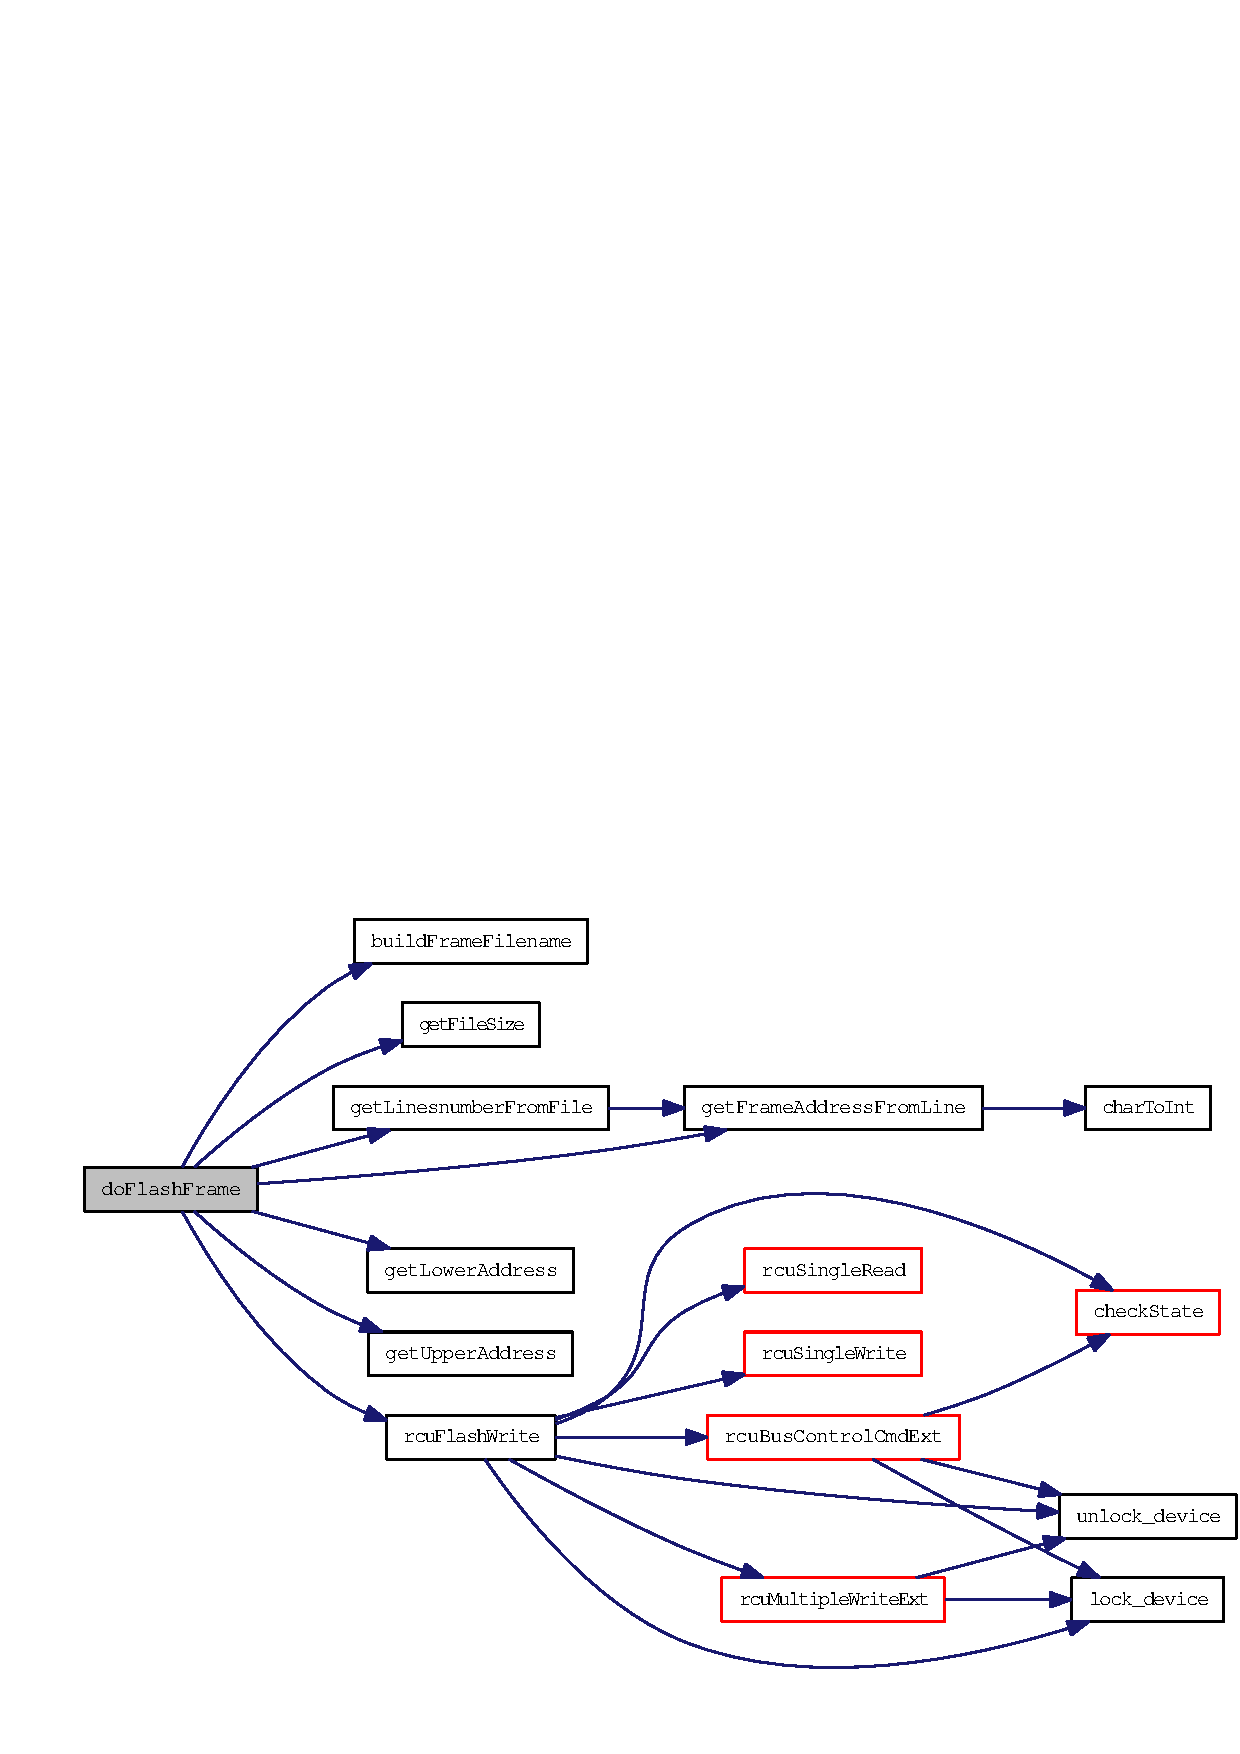
\includegraphics[width=299pt]{rcuflashprog_8c_237fcbe3877916a856ff7acf973ee2ba_cgraph}
\end{center}
\end{figure}
\hypertarget{rcuflashprog_8c_017730762068a4d5359376e97dac8257}{
\index{rcuflashprog.c@{rcuflashprog.c}!doInit@{doInit}}
\index{doInit@{doInit}!rcuflashprog.c@{rcuflashprog.c}}
\subsubsection[doInit]{\setlength{\rightskip}{0pt plus 5cm}int do\-Init (char $\ast$ {\em conffilename}, int {\em BB\_\-FLASH})}}
\label{rcuflashprog_8c_017730762068a4d5359376e97dac8257}




Definition at line 842 of file rcuflashprog.c.

References calculate\-Stop\-Address(), EXIT\_\-FAILURE, get\-File\-Size(), get\-Lower\-Address(), get\-Upper\-Address(), rcu\-Flash\-Write(), and TRUE.

Referenced by main().

Here is the call graph for this function:\begin{figure}[H]
\begin{center}
\leavevmode
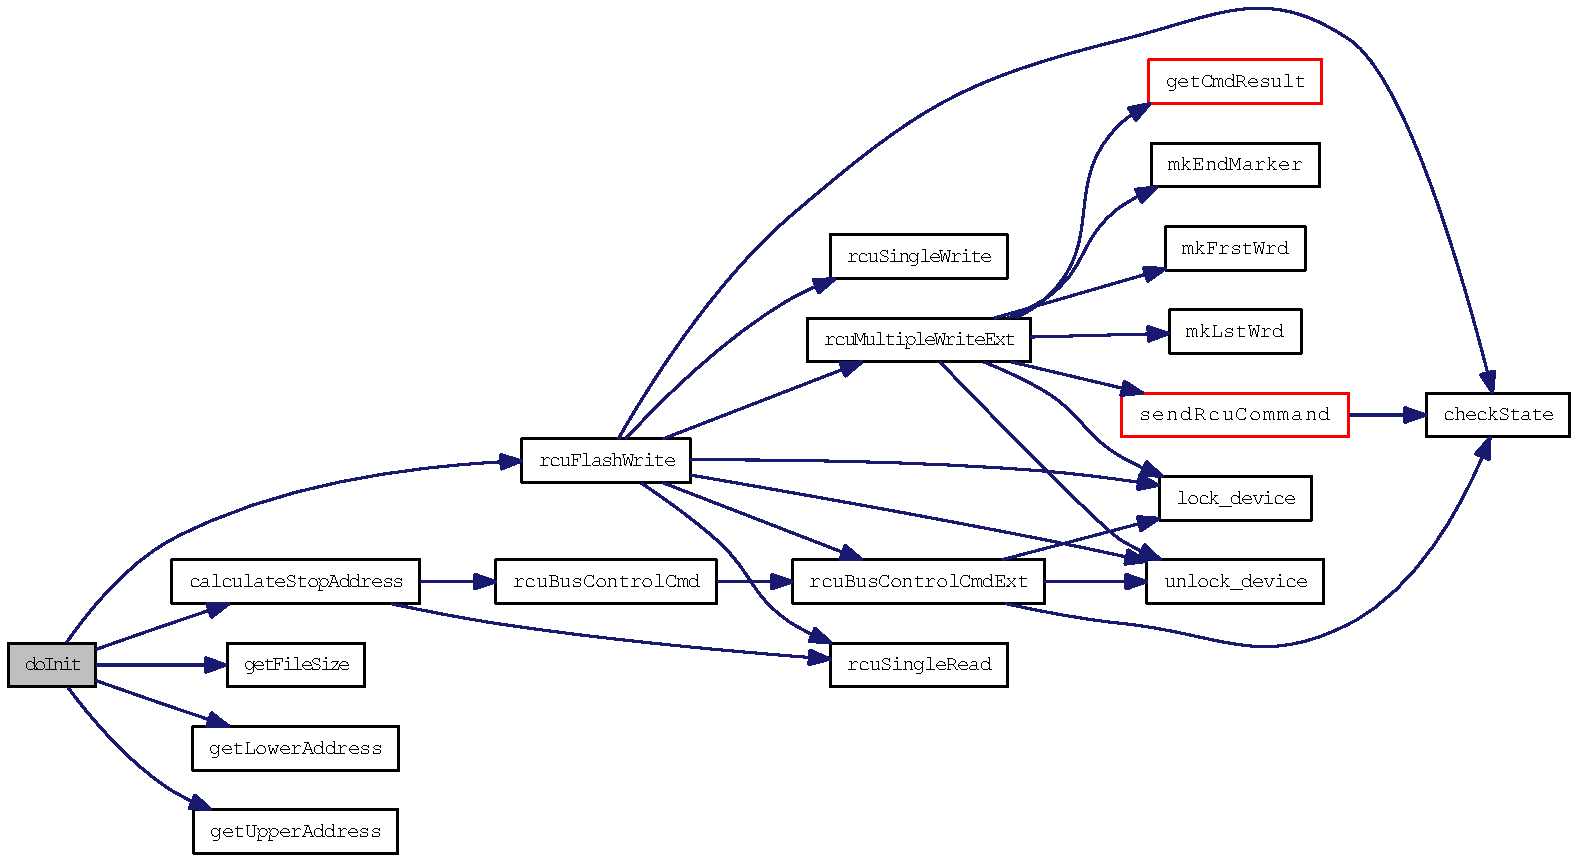
\includegraphics[width=397pt]{rcuflashprog_8c_017730762068a4d5359376e97dac8257_cgraph}
\end{center}
\end{figure}
\hypertarget{rcuflashprog_8c_cd9a55766b840c98d87b0ce1a76af867}{
\index{rcuflashprog.c@{rcuflashprog.c}!doScrubbing@{doScrubbing}}
\index{doScrubbing@{doScrubbing}!rcuflashprog.c@{rcuflashprog.c}}
\subsubsection[doScrubbing]{\setlength{\rightskip}{0pt plus 5cm}int do\-Scrubbing (char $\ast$ {\em conffilename}, int {\em BB\_\-FLASH})}}
\label{rcuflashprog_8c_cd9a55766b840c98d87b0ce1a76af867}


Everything needed for a complete scrubbing is done here. 

All necessary Information is read out from the given configfile.

\begin{Desc}
\item[Returns:]not used \end{Desc}


Definition at line 649 of file rcuflashprog.c.

References calculate\-Stop\-Address(), EXIT\_\-FAILURE, get\-File\-Size(), get\-Lower\-Address(), get\-Upper\-Address(), rcu\-Flash\-Write(), and TRUE.

Referenced by main().

Here is the call graph for this function:\begin{figure}[H]
\begin{center}
\leavevmode
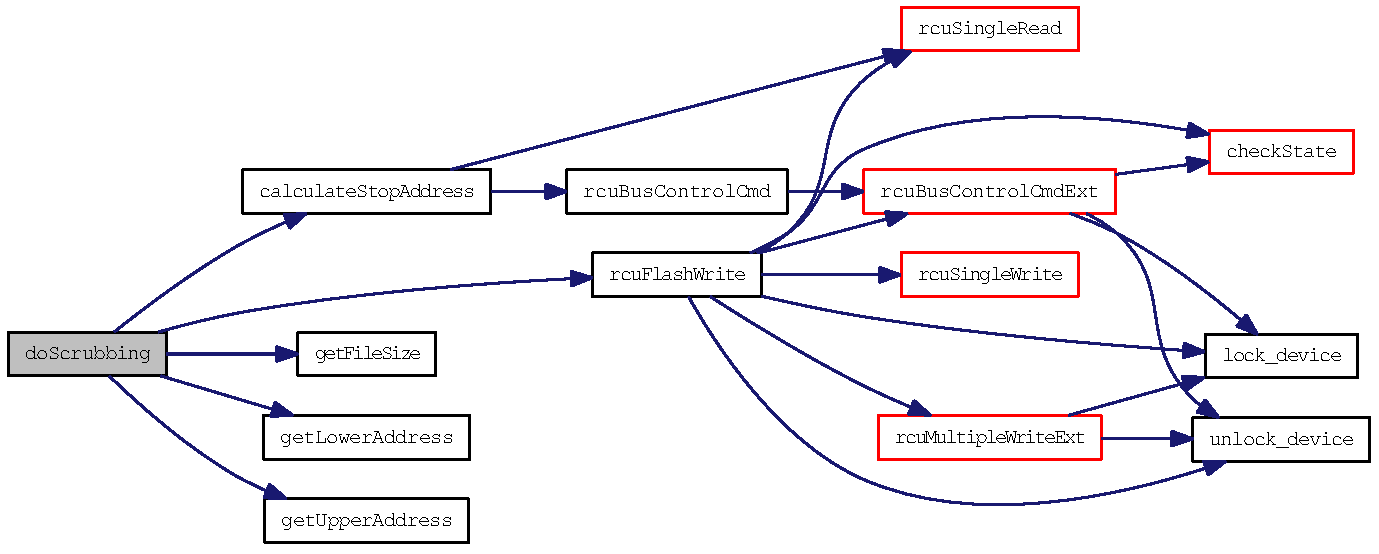
\includegraphics[width=349pt]{rcuflashprog_8c_cd9a55766b840c98d87b0ce1a76af867_cgraph}
\end{center}
\end{figure}
\hypertarget{rcuflashprog_8c_3c04138a5bfe5d72780bb7e82a18e627}{
\index{rcuflashprog.c@{rcuflashprog.c}!main@{main}}
\index{main@{main}!rcuflashprog.c@{rcuflashprog.c}}
\subsubsection[main]{\setlength{\rightskip}{0pt plus 5cm}int main (int {\em argc}, char $\ast$$\ast$ {\em argv})}}
\label{rcuflashprog_8c_3c04138a5bfe5d72780bb7e82a18e627}




Definition at line 43 of file rcuflashprog.c.

References BB\_\-FLASH, do\-Flash\-Frame(), do\-Init(), do\-Scrubbing(), enter\-Flash\-State(), EXIT\_\-FAILURE, FALSE, get\-Bus\-State(), init(), init\-Rcu\-Access(), rcu\-Flash\-Erase(), rcu\-Single\-Write(), release\-Rcu\-Access(), restore\-Bus\-State(), and TRUE.

Here is the call graph for this function:\begin{figure}[H]
\begin{center}
\leavevmode
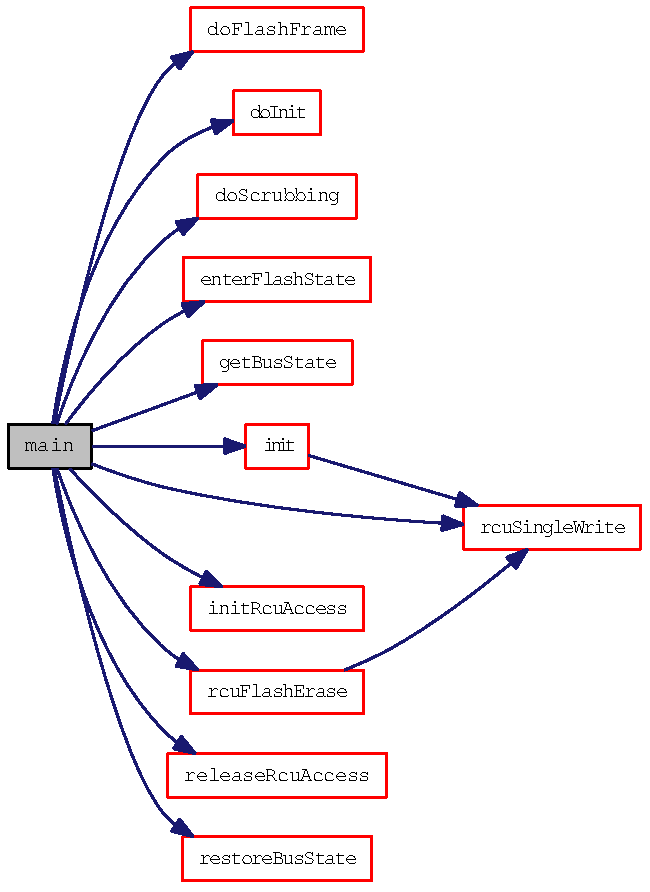
\includegraphics[width=174pt]{rcuflashprog_8c_3c04138a5bfe5d72780bb7e82a18e627_cgraph}
\end{center}
\end{figure}


\subsection{Variable Documentation}
\hypertarget{rcuflashprog_8c_a1aabbeb0deebd40a25e329692500bbe}{
\index{rcuflashprog.c@{rcuflashprog.c}!BB_FLASH@{BB\_\-FLASH}}
\index{BB_FLASH@{BB\_\-FLASH}!rcuflashprog.c@{rcuflashprog.c}}
\subsubsection[BB\_\-FLASH]{\setlength{\rightskip}{0pt plus 5cm}int \hyperlink{rcuflashprog_8c_a1aabbeb0deebd40a25e329692500bbe}{BB\_\-FLASH}\hspace{0.3cm}{\tt  \mbox{[}static\mbox{]}}}}
\label{rcuflashprog_8c_a1aabbeb0deebd40a25e329692500bbe}




Definition at line 41 of file rcuflashprog.c.

Referenced by main().